\chapter{Test chapter}

So far we have been limited in which objects we can manipulate and intersect
in CGA. Specifically we can only deal with planes, circles, spheres, lines and
points. In this section we consider a method of extending our approach to
conics and intersections thereof. We shall proceed by considering the 
3-dimensional Euclidean case but this method may be generalised to higher
dimensions if required; here we follow the procedure outlined in
\cite{anthonyChina}.
We shall begin by considering the set of points on the unit sphere at the 
origin:
\[
\left\{ c_\theta e_1 + s_\theta c_\phi e_2 + s_\theta c_\phi e_3\,:\,
	\theta \in (0,2\pi],\,\phi \in (0,\pi] \right\}
\]
where $c_\theta = \cos(\theta)$, $s_\theta = \sin(\theta)$ and similarly
for $s_\phi$ and $c_\phi$. We apply the transform $F(\cdot)$ to
obtain the set, $S$, of representations for these points:
\[
S = \left\{ \frac{n}{2} + c_\theta e_1 + s_\theta c_\phi e_2
+ s_\theta c_\phi e_3 -
    \frac{\bar{n}}{2} \,:\,
	\theta \in (0,2\pi],\,\phi \in (0,\pi] \right\}
\]
and consider the effect of the transform from \cite{anthonyChina} below 
\[
C_\alpha(X) = \beta \left[ X + \frac{\alpha}{2} (X \cdot e_1) \wedge \bar{n} \right]
\]
which we shall term the \emph{conic transform}, upon the elements of $S$ 
where $\beta$ is chosen so that our normalisation constraint
$C_\alpha(X) \cdot n = -1$ still holds:
\[
\{ C_\alpha(X) : X \in S \} \equiv \left\{ \frac{1}{1 - \alpha \cos \theta} \left(
	\frac{n}{2} + c_\theta e_1 + s_\theta c_\phi e_2 
              + s_\theta c_\phi e_3 \right) -
    \frac{\bar{n}}{2} \,:\,
	\theta \in (0,2\pi],\,\phi \in (0,\pi] \right\}
\]

\section{Test section}

The elements of this set are no-longer null-vectors (they have extra
components parallel to $n$) but one may still apply the inverse
mapping $F^{-1}(\cdot)$ and extract a spatial vector (i.e.\ 
one with no components parallel to $e$ or $\bar{e}$). It is found
\cite{anthonyChina, jic23fyr} that the spatial vectors extracted thus lie
on the surface of a quadric with a rotational cross-section corresponding
to a conic. The form of this conic cross-section is determined by the
parameter $\alpha$ which can be interpreted as the
eccentricity:
\begin{itemize}
\item $\alpha = 0$ : The set of points lie on the unit sphere.
\item $0 < \alpha < 1$ : The set of points lie on an ellipsoid formed
by rotating an ellipse in the $e_{12}$ plane about $e_1$. The origin
lies at one of the foci and $\alpha$ is the eccentricity.
\item $\alpha = 1$ : The set of points lie on a paraboloid specified
by the points 
\[\{ x : 2 x\cdot e_1 = [(x \cdot e_2)^2 + (x \cdot e_3)^2] -1\}.\]
\item $\alpha > 1$ : The set of points lie on a two-sheeted hyperboloid formed
by rotating an hyperbola in the $e_{12}$ plane about $e_1$. The origin
is once again one of the foci and the eccentricity is $\alpha$.
\end{itemize}
We may therefore form a set of representations for points lying on 
these conics by simply applying appropriate translation,
dilation and rotation rotors after the conic transform.

\subsection{Properties of the conic transform}

It can further be shown \cite{jic23fyr} that the conic transform preserves
the outer product but not the inner (and hence geometric) products. That
is to say $C_\alpha(X \wedge Y) = C_\alpha(X) \wedge C_\alpha(Y)$. It also preserves the 
`special' vectors $n$ and $\bar{n}$. From this we can easily show that
$C_\alpha(\cdot)$ does not change the nature of `flat' objects 
(i.e.\ planes and lines transform to other planes and
 lines) since
\begin{eqnarray*}
C_\alpha\left(X_1 \wedge X_2 \wedge \cdots \wedge X_i \wedge n \right) & = &
C_\alpha(X_1) \wedge C_\alpha(X_2) \wedge \cdots \wedge C_\alpha(X_i) \wedge C_\alpha(n) \\
&=& C_\alpha(X_1) \wedge C_\alpha(X_2) \wedge \cdots \wedge C_\alpha(X_i) \wedge n.
\end{eqnarray*}

It is also easy to verify by direct substitution
that the conic transform preserves direction of points from the
origin, i.e.\ that
\[
F^{-1}(C_\alpha(F( a_ie_i ))) =
	 \frac{a_i}{1 - \alpha a_1} e_i
\]
where we have adopted the usual summation convention.

\subsection{Intersections}

We may now consider how to apply this transform to intersecting conics
with lines. Suppose that we have found a rotor $R$ and value of 
$\alpha$ such that the set of points represented by
\[
\{ RC_\alpha(X)\tilde{R}\,:\,X \in S\}
\]
lie on the conic we wish to intersect. Suppose further that we wish to 
intersect it with the line represented by the trivector $L$ (as in
figure \ref{fig:conic_transform}a). We shall denote the 
points of intersection $A$ and $B$. Now consider
the effect of applying $C_\alpha^{-1}(\tilde{R} X R)$ to each of our 
objects and
points (where $X$ is the appropriate object). 
The points on the conic are transformed to the unit sphere. The line, $L$,
is transformed to $C_\alpha^{-1}(\tilde{R}LR)$ (figure \ref{fig:conic_transform}) which is still a line since the
conic transform maps lines to lines. 
The points of intersection between
this new line and our unit sphere may be found via the usual meet
formulation:
\[
A' \wedge B' = \Sigma \vee C_\alpha^{-1}(\tilde{R}LR)
\]
where $\Sigma$ is the multivector representing the unit sphere which may
be formed as 
\[
\Sigma = F(e_1) \wedge F(e_2) \wedge F(e_3) \wedge F(-e_1) % \equiv F(-e_{23})
\]
or similar.

\begin{figure}[t]\centering
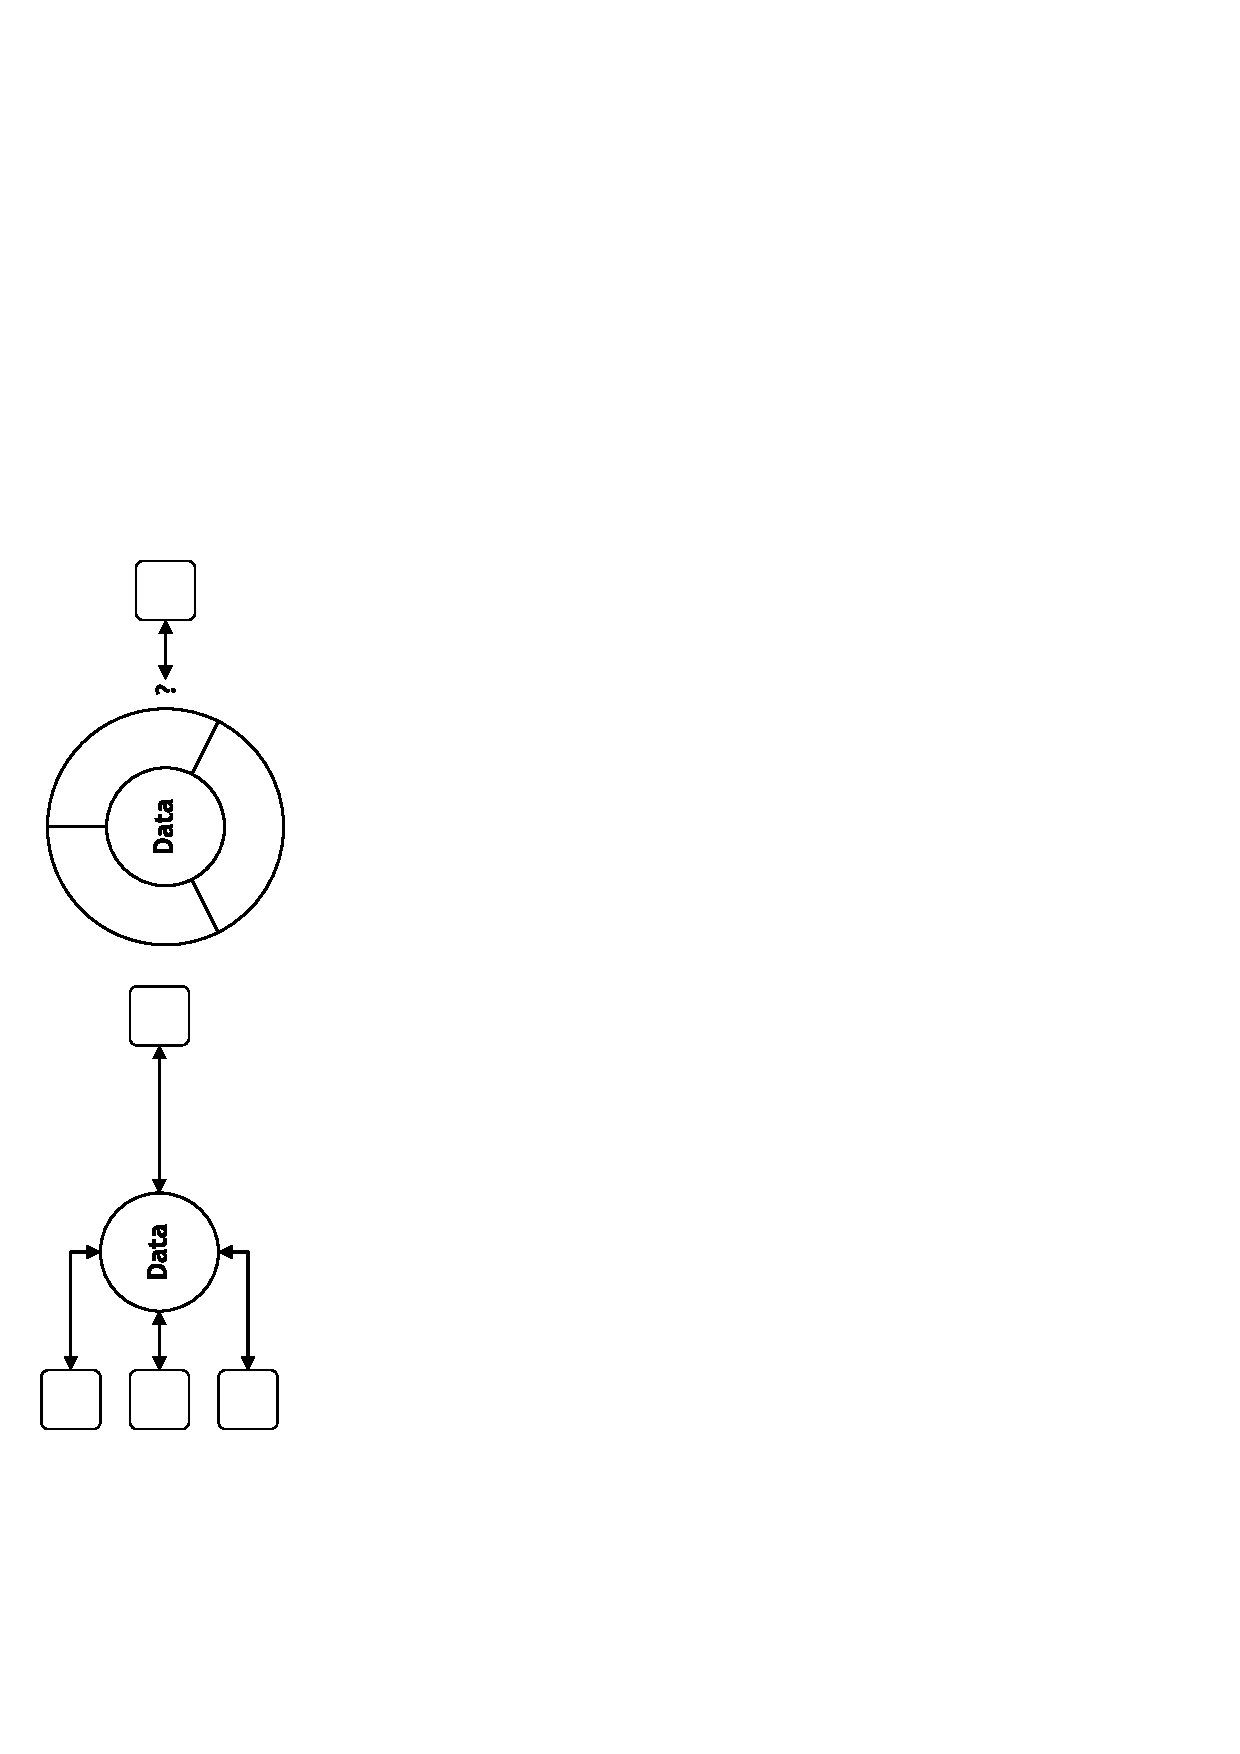
\includegraphics[width=0.8\columnwidth]{diagram1}
\caption{\label{fig:conic_transform}Intersection of line $L$ with 
  (a) conic and (b) transformation back to intersection with unit sphere.}
\end{figure}

Finally we consider the transformed points $A = RC_\alpha(A')\tilde{R}$
and
$B = RC_\alpha(B')\tilde{R}$. They must lie upon our original line 
$L$ since
$A'$ and $B'$ clearly lie on $C_\alpha^{-1}(\tilde{R}LR)$ and 
\[ RC_\alpha(C_\alpha^{-1}(\tilde{R}LR))\tilde{R} = L. \]
They must also lie upon our conic since $A'$ and $B'$ lie on the unit sphere
and the transformation is exactly that which generated our original conic.
If they lie upon our conic and upon $L$ they must therefore be the points
of intersection.
We have therefore formulated a method for intersecting lines and conics. 

\subsection{Reflections}
\label{sec:Ref}
We now consider the reflection of rays from conics. In order to
reflect a ray we wish to find the tangent plane for a conic at the 
intersection point of the incoming ray with the conic. Again we
make use of the fact that $C_\alpha(\cdot)$ maps planes to
planes and apply $C_\alpha^{-1}(\tilde{R}XR)$ to all objects moving the
points on the conic to the unit sphere. We then find the intersection
point and tangent plane for the unit sphere. It can be shown \cite{jic23fyr}
that when transformed back via $RC_\alpha(\cdot)\tilde{R}$ the tangent
plane of the sphere maps to the tangent plane for the conic. Reflection
can then be performed by simply reflecting the incoming ray $L$ in
this plane, $\Phi$:
\[
L' = \Phi L \Phi.
\]
\section{Line Images in a Para-catadioptric Camera}
\begin{figure}[ht]
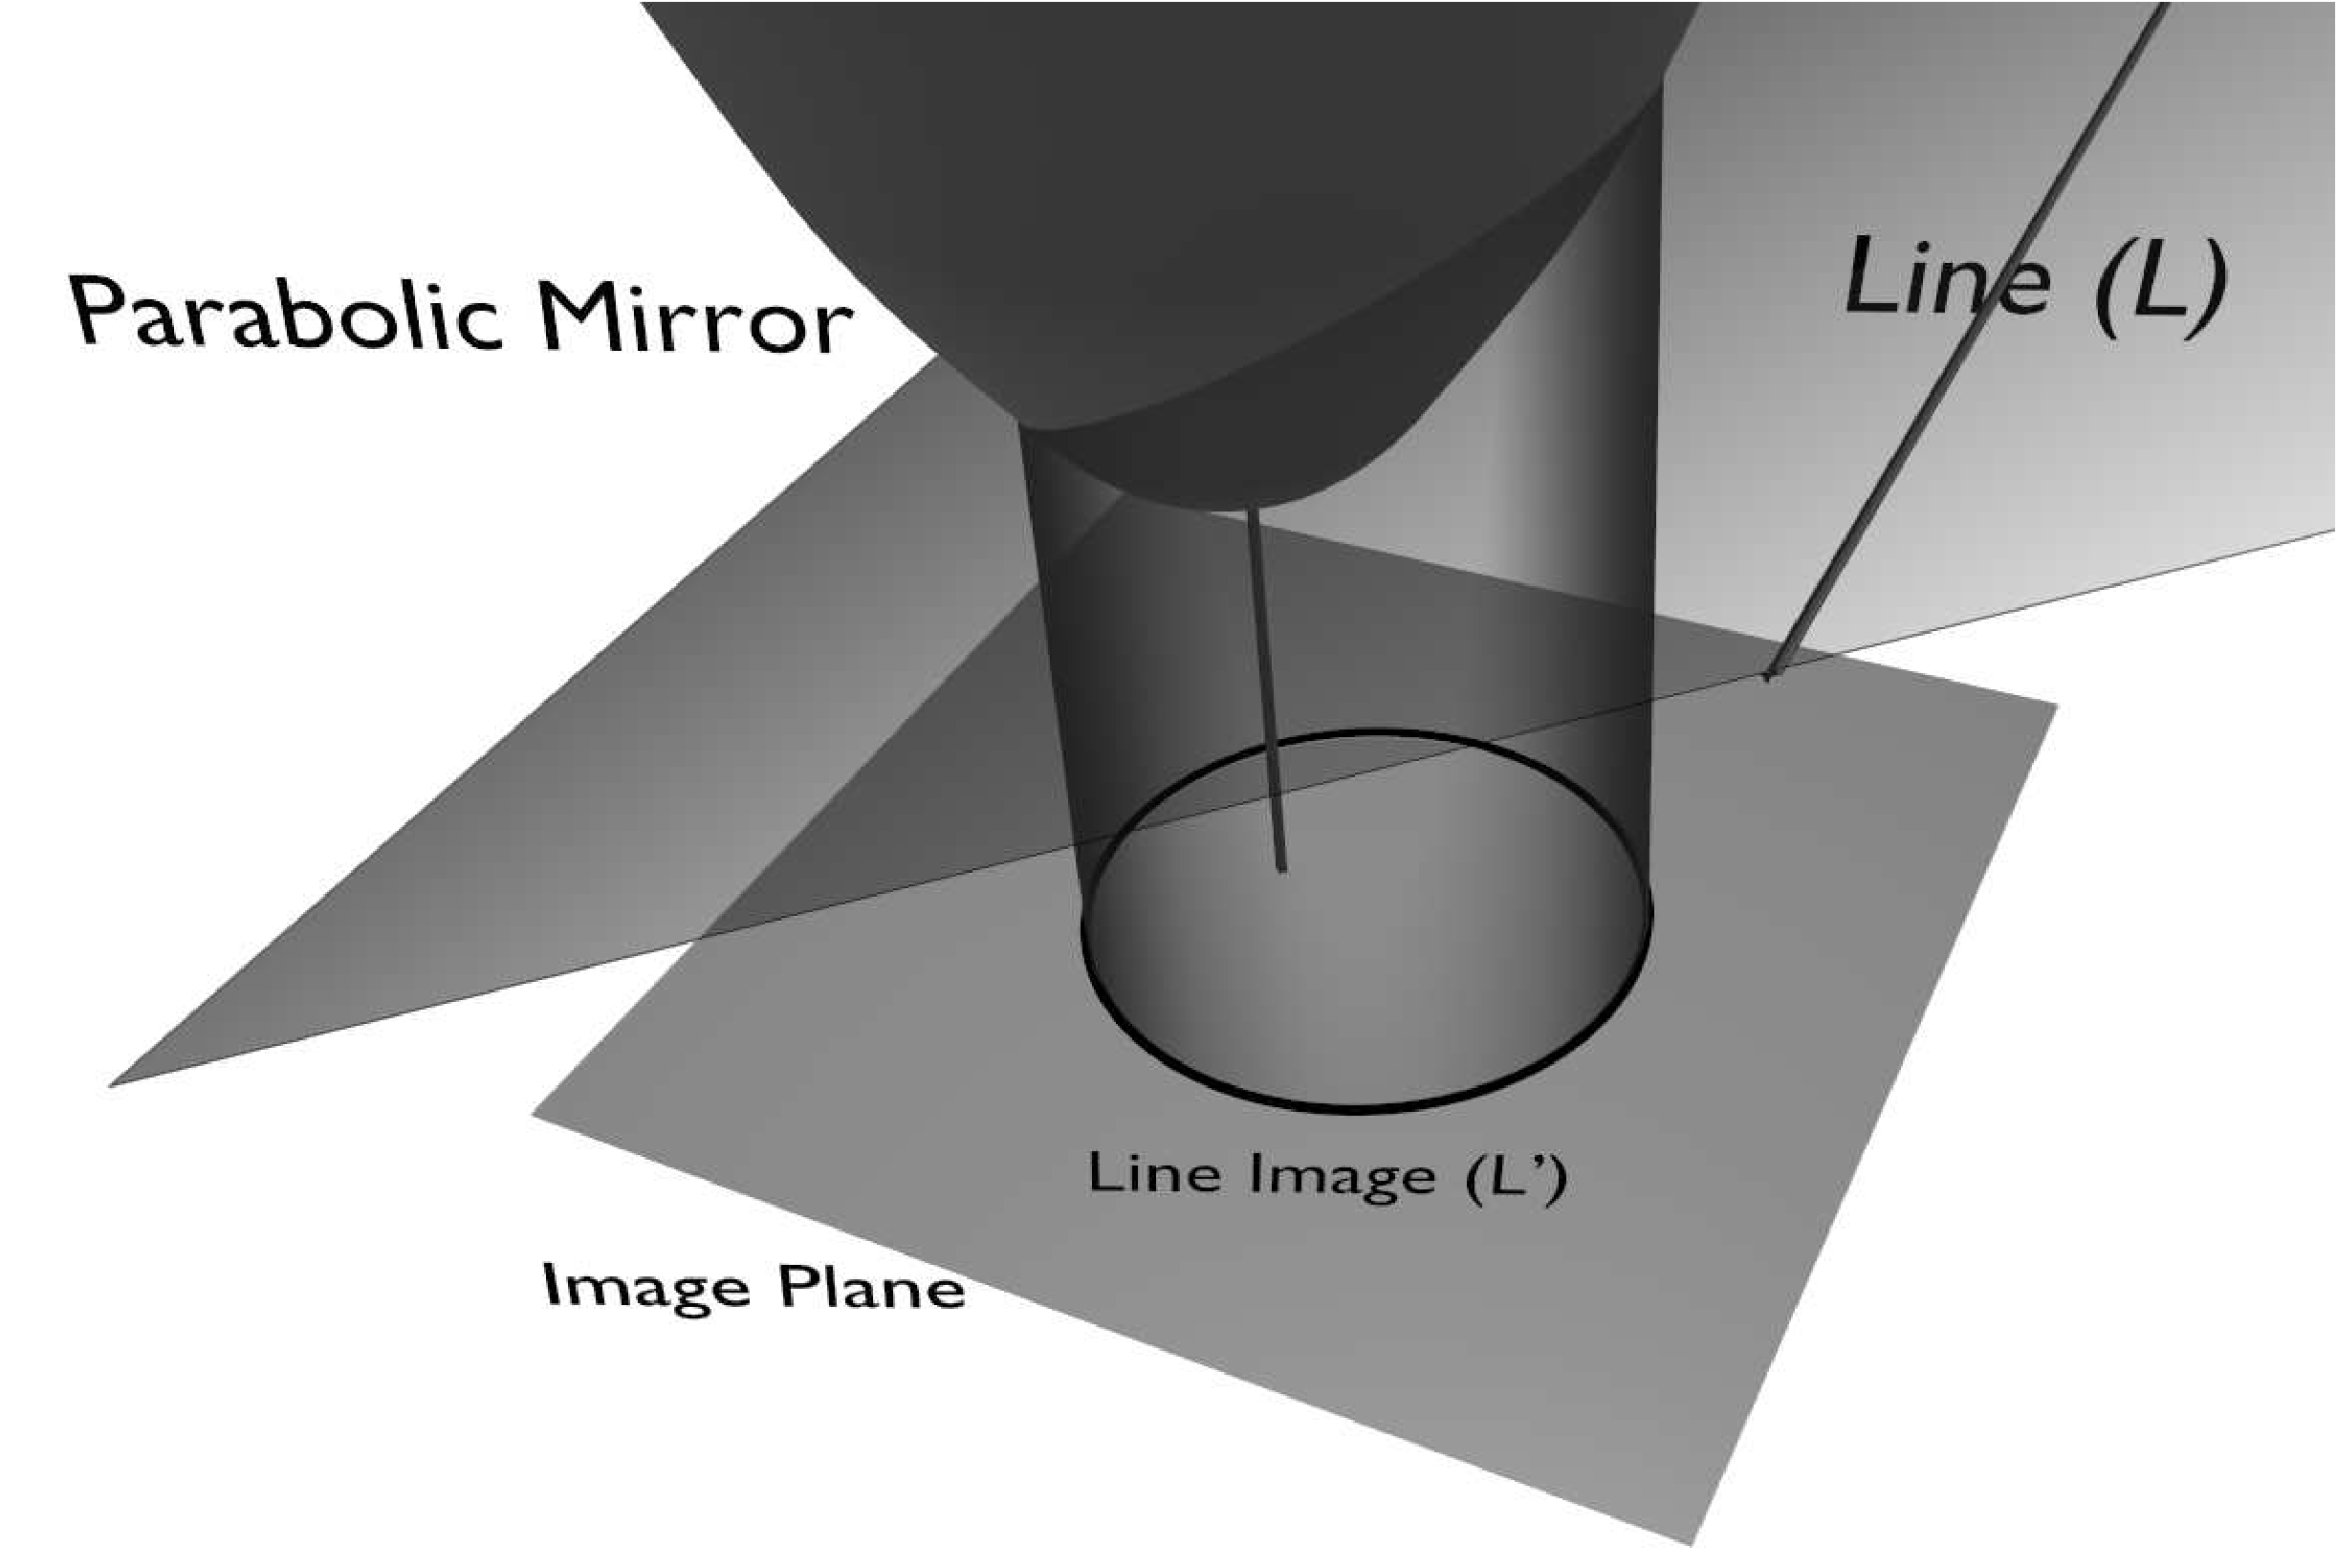
\includegraphics[height=8cm]{testparaboloid2}
\caption{Para-catadioptric Line Image Formation}
\label{fig:bob}
\end{figure}
As an illustration of the power of the techniques described above, let us consider the simple but
 useful question of what the image of a straight line in a parabolic mirror based Single View Point 
catadioptric (SVP Para-catadioptric) camera is.  This problem has been considered in a number 
of papers e.g.\ \cite{CAM:gd, CAM:YH04, CAM:BA03b, CAM:bclf} and is useful for calibration 
and scene reconstruction.

The setup in question is illustated in figure \ref{fig:bob}. With a parabolic
mirror the SVP constraint requires that all the rays from the mirror imaged by
the camera are parallel to the mirror axis and hence the camera is
orthographic. Let us consider the source of light forming an image at the point
$xe_2 + ye_3$.  As we are imaging with an orthographic camera, for the setup
shown, this ray is in the $e_1$ direction, which is axis of both the camera and the parabolic mirror.  The focus of the parabolic mirror is situated at the origin. 
\begin{eqnarray}  
S_1&=& \left[e_{23} + (xe_3 - ye_2)n\right]^* \nonumber
\end{eqnarray} 
This result is easily established if we consider the form of the dual of a line \cite{cgwcga}.
\begin{eqnarray}
L^* &=&	\hat{m}I_3 + [(a\wedge \hat{m})I_3]n\nonumber
\end{eqnarray}
with $\hat{m} = e_1$ (the ray's direction), $a = xe_2 + ye_3$ (a point on the ray) and $I_3 = e_{123}$.
This form is analogous to writing the line in terms of Pl\"{u}cker coordinates where 3 of the coordinates give the line's direction and the other 3 give its moment about the origin.



We are interested in the reflection of this ray in the mirror.  This reflected ray, $S_2$ is found as
described in Section \ref{sec:Ref}.  
\begin{eqnarray} 
\label{eq:1} 
S_2 &=& \frac{1-x^2-y^2}2e_{145} -xe_{245} - y e_{345} 
\end{eqnarray}  
For this ray to be the image ray of a point on a line $L$ they must intersect and hence
\begin{eqnarray} 
\label{eq:2} L\vee S_2 &=& 0 
\end{eqnarray} 
As stated above, a line, $L$, with unit direction vector $\hat{m} = m_1e_1 + m_2e_2 + m_3e_3$ (such that $\hat{m}^2 = 1$) passing through the point $a = a_1e_1 + a_2e_2 + a_3e_3$, can be expressed as 
\begin{eqnarray} 
\label{eq:3} L &=& \left[\hat{m}I_3 + ((a\wedge \hat{m})I_3)n\right]^* 
\end{eqnarray} 

Subsituting equations \ref{eq:3} and \ref{eq:1} into \ref{eq:2} and rearranging, the condition obtained is 
\begin{eqnarray}
  \left(x + \frac{a_3m_1 - a_1m_3}{a_2m_3 -a_3m_2}\right)^2 + \left(y + \frac{a_1m_2 - a_2m_1}{a_2m_3 - a_3m_2}\right)^2 \nonumber&&\\- \left(1 + \left(\frac{a_3m_1 - a_1m_3}{a_2m_3 - a3_m2}\right)^2 + \left(\frac{a_1m_2 - a_2m_1}{a_2m_3 -a_3m_2}\right)^2\right) &=& 0
\end{eqnarray} 
As others have observed \cite{CAM:gd}, this is a circle ($L'$ in figure
		\ref{fig:bob}). A similar derivation can be used to establish
the image of a sphere in such a camera the only significant change being that
the resulting condition is the product of two separate circle equations,
    indicating an ambiguity which can trivially be resolved.  \nocite{CAM:bclf}

\chapter*{Test starred chapter}

So far we have been limited in which objects we can manipulate and intersect
in CGA. Specifically we can only deal with planes, circles, spheres, lines and
points. In this section we consider a method of extending our approach to
conics and intersections thereof. We shall proceed by considering the 
3-dimensional Euclidean case but this method may be generalised to higher
dimensions if required; here we follow the procedure outlined in
\cite{anthonyChina}.
We shall begin by considering the set of points on the unit sphere at the 
origin:
\[
\left\{ c_\theta e_1 + s_\theta c_\phi e_2 + s_\theta c_\phi e_3\,:\,
	\theta \in (0,2\pi],\,\phi \in (0,\pi] \right\}
\]
where $c_\theta = \cos(\theta)$, $s_\theta = \sin(\theta)$ and similarly
for $s_\phi$ and $c_\phi$. We apply the transform $F(\cdot)$ to
obtain the set, $S$, of representations for these points:
\[
S = \left\{ \frac{n}{2} + c_\theta e_1 + s_\theta c_\phi e_2
+ s_\theta c_\phi e_3 -
    \frac{\bar{n}}{2} \,:\,
	\theta \in (0,2\pi],\,\phi \in (0,\pi] \right\}
\]
and consider the effect of the transform from \cite{anthonyChina} below 
\[
C_\alpha(X) = \beta \left[ X + \frac{\alpha}{2} (X \cdot e_1) \wedge \bar{n} \right]
\]
which we shall term the \emph{conic transform}, upon the elements of $S$ 
where $\beta$ is chosen so that our normalisation constraint
$C_\alpha(X) \cdot n = -1$ still holds:
\[
\{ C_\alpha(X) : X \in S \} \equiv \left\{ \frac{1}{1 - \alpha \cos \theta} \left(
	\frac{n}{2} + c_\theta e_1 + s_\theta c_\phi e_2 
              + s_\theta c_\phi e_3 \right) -
    \frac{\bar{n}}{2} \,:\,
	\theta \in (0,2\pi],\,\phi \in (0,\pi] \right\}
\]

\chapter{Another Test Chapter --- This time we will use a very long title
and see how wrapping works}

So far we have been limited in which objects we can manipulate and intersect
in CGA. Specifically we can only deal with planes, circles, spheres, lines and
points. In this section we consider a method of extending our approach to
conics and intersections thereof. We shall proceed by considering the 
3-dimensional Euclidean case but this method may be generalised to higher
dimensions if required; here we follow the procedure outlined in
\cite{anthonyChina}.
We shall begin by considering the set of points on the unit sphere at the 
origin:
\[
\left\{ c_\theta e_1 + s_\theta c_\phi e_2 + s_\theta c_\phi e_3\,:\,
	\theta \in (0,2\pi],\,\phi \in (0,\pi] \right\}
\]
where $c_\theta = \cos(\theta)$, $s_\theta = \sin(\theta)$ and similarly
for $s_\phi$ and $c_\phi$. We apply the transform $F(\cdot)$ to
obtain the set, $S$, of representations for these points:
\[
S = \left\{ \frac{n}{2} + c_\theta e_1 + s_\theta c_\phi e_2
+ s_\theta c_\phi e_3 -
    \frac{\bar{n}}{2} \,:\,
	\theta \in (0,2\pi],\,\phi \in (0,\pi] \right\}
\]
and consider the effect of the transform from \cite{anthonyChina} below 
\[
C_\alpha(X) = \beta \left[ X + \frac{\alpha}{2} (X \cdot e_1) \wedge \bar{n} \right]
\]
which we shall term the \emph{conic transform}, upon the elements of $S$ 
where $\beta$ is chosen so that our normalisation constraint
$C_\alpha(X) \cdot n = -1$ still holds:
\[
\{ C_\alpha(X) : X \in S \} \equiv \left\{ \frac{1}{1 - \alpha \cos \theta} \left(
	\frac{n}{2} + c_\theta e_1 + s_\theta c_\phi e_2 
              + s_\theta c_\phi e_3 \right) -
    \frac{\bar{n}}{2} \,:\,
	\theta \in (0,2\pi],\,\phi \in (0,\pi] \right\}
\]

\section{Test section}

The elements of this set are no-longer null-vectors (they have extra
components parallel to $n$) but one may still apply the inverse
mapping $F^{-1}(\cdot)$ and extract a spatial vector (i.e.\ 
one with no components parallel to $e$ or $\bar{e}$). It is found
\cite{anthonyChina, jic23fyr} that the spatial vectors extracted thus lie
on the surface of a quadric with a rotational cross-section corresponding
to a conic. The form of this conic cross-section is determined by the
parameter $\alpha$ which can be interpreted as the
eccentricity:
\begin{itemize}
\item $\alpha = 0$ : The set of points lie on the unit sphere.
\item $0 < \alpha < 1$ : The set of points lie on an ellipsoid formed
by rotating an ellipse in the $e_{12}$ plane about $e_1$. The origin
lies at one of the foci and $\alpha$ is the eccentricity.
\item $\alpha = 1$ : The set of points lie on a paraboloid specified
by the points 
\[\{ x : 2 x\cdot e_1 = [(x \cdot e_2)^2 + (x \cdot e_3)^2] -1\}.\]
\item $\alpha > 1$ : The set of points lie on a two-sheeted hyperboloid formed
by rotating an hyperbola in the $e_{12}$ plane about $e_1$. The origin
is once again one of the foci and the eccentricity is $\alpha$.
\end{itemize}
We may therefore form a set of representations for points lying on 
these conics by simply applying appropriate translation,
dilation and rotation rotors after the conic transform.

\subsection{Properties of the conic transform}

It can further be shown \cite{jic23fyr} that the conic transform preserves
the outer product but not the inner (and hence geometric) products. That
is to say $C_\alpha(X \wedge Y) = C_\alpha(X) \wedge C_\alpha(Y)$. It also preserves the 
`special' vectors $n$ and $\bar{n}$. From this we can easily show that
$C_\alpha(\cdot)$ does not change the nature of `flat' objects 
(i.e.\ planes and lines transform to other planes and
 lines) since
\begin{eqnarray*}
C_\alpha\left(X_1 \wedge X_2 \wedge \cdots \wedge X_i \wedge n \right) & = &
C_\alpha(X_1) \wedge C_\alpha(X_2) \wedge \cdots \wedge C_\alpha(X_i) \wedge C_\alpha(n) \\
&=& C_\alpha(X_1) \wedge C_\alpha(X_2) \wedge \cdots \wedge C_\alpha(X_i) \wedge n.
\end{eqnarray*}

It is also easy to verify by direct substitution
that the conic transform preserves direction of points from the
origin, i.e.\ that
\[
F^{-1}(C_\alpha(F( a_ie_i ))) =
	 \frac{a_i}{1 - \alpha a_1} e_i
\]
where we have adopted the usual summation convention.

\subsection{Intersections}

We may now consider how to apply this transform to intersecting conics
with lines. Suppose that we have found a rotor $R$ and value of 
$\alpha$ such that the set of points represented by
\[
\{ RC_\alpha(X)\tilde{R}\,:\,X \in S\}
\]
lie on the conic we wish to intersect. Suppose further that we wish to 
intersect it with the line represented by the trivector $L$ (as in
figure \ref{fig:conic_transform}a). We shall denote the 
points of intersection $A$ and $B$. Now consider
the effect of applying $C_\alpha^{-1}(\tilde{R} X R)$ to each of our 
objects and
points (where $X$ is the appropriate object). 
The points on the conic are transformed to the unit sphere. The line, $L$,
is transformed to $C_\alpha^{-1}(\tilde{R}LR)$ (figure \ref{fig:conic_transform}) which is still a line since the
conic transform maps lines to lines. 
The points of intersection between
this new line and our unit sphere may be found via the usual meet
formulation:
\[
A' \wedge B' = \Sigma \vee C_\alpha^{-1}(\tilde{R}LR)
\]
where $\Sigma$ is the multivector representing the unit sphere which may
be formed as 
\[
\Sigma = F(e_1) \wedge F(e_2) \wedge F(e_3) \wedge F(-e_1) % \equiv F(-e_{23})
\]
or similar.

\begin{figure}[t]\centering
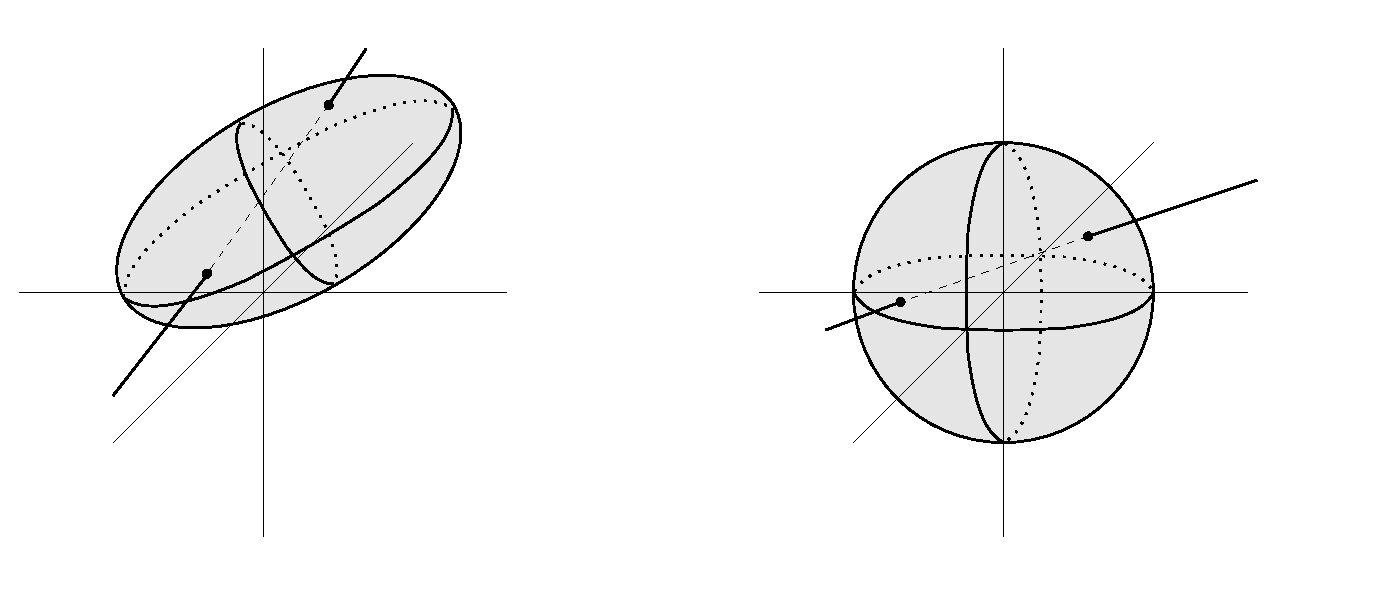
\includegraphics[width=0.8\columnwidth]{conic_transform}
\caption{\label{fig:conic_transform}Intersection of line $L$ with 
  (a) conic and (b) transformation back to intersection with unit sphere.}
\end{figure}

Finally we consider the transformed points $A = RC_\alpha(A')\tilde{R}$
and
$B = RC_\alpha(B')\tilde{R}$. They must lie upon our original line 
$L$ since
$A'$ and $B'$ clearly lie on $C_\alpha^{-1}(\tilde{R}LR)$ and 
\[ RC_\alpha(C_\alpha^{-1}(\tilde{R}LR))\tilde{R} = L. \]
They must also lie upon our conic since $A'$ and $B'$ lie on the unit sphere
and the transformation is exactly that which generated our original conic.
If they lie upon our conic and upon $L$ they must therefore be the points
of intersection.
We have therefore formulated a method for intersecting lines and conics. 

\subsection{Reflections}
\label{sec:Ref}
We now consider the reflection of rays from conics. In order to
reflect a ray we wish to find the tangent plane for a conic at the 
intersection point of the incoming ray with the conic. Again we
make use of the fact that $C_\alpha(\cdot)$ maps planes to
planes and apply $C_\alpha^{-1}(\tilde{R}XR)$ to all objects moving the
points on the conic to the unit sphere. We then find the intersection
point and tangent plane for the unit sphere. It can be shown \cite{jic23fyr}
that when transformed back via $RC_\alpha(\cdot)\tilde{R}$ the tangent
plane of the sphere maps to the tangent plane for the conic. Reflection
can then be performed by simply reflecting the incoming ray $L$ in
this plane, $\Phi$:
\[
L' = \Phi L \Phi.
\]
\section{Line Images in a Para-catadioptric Camera}
\begin{figure}[ht]
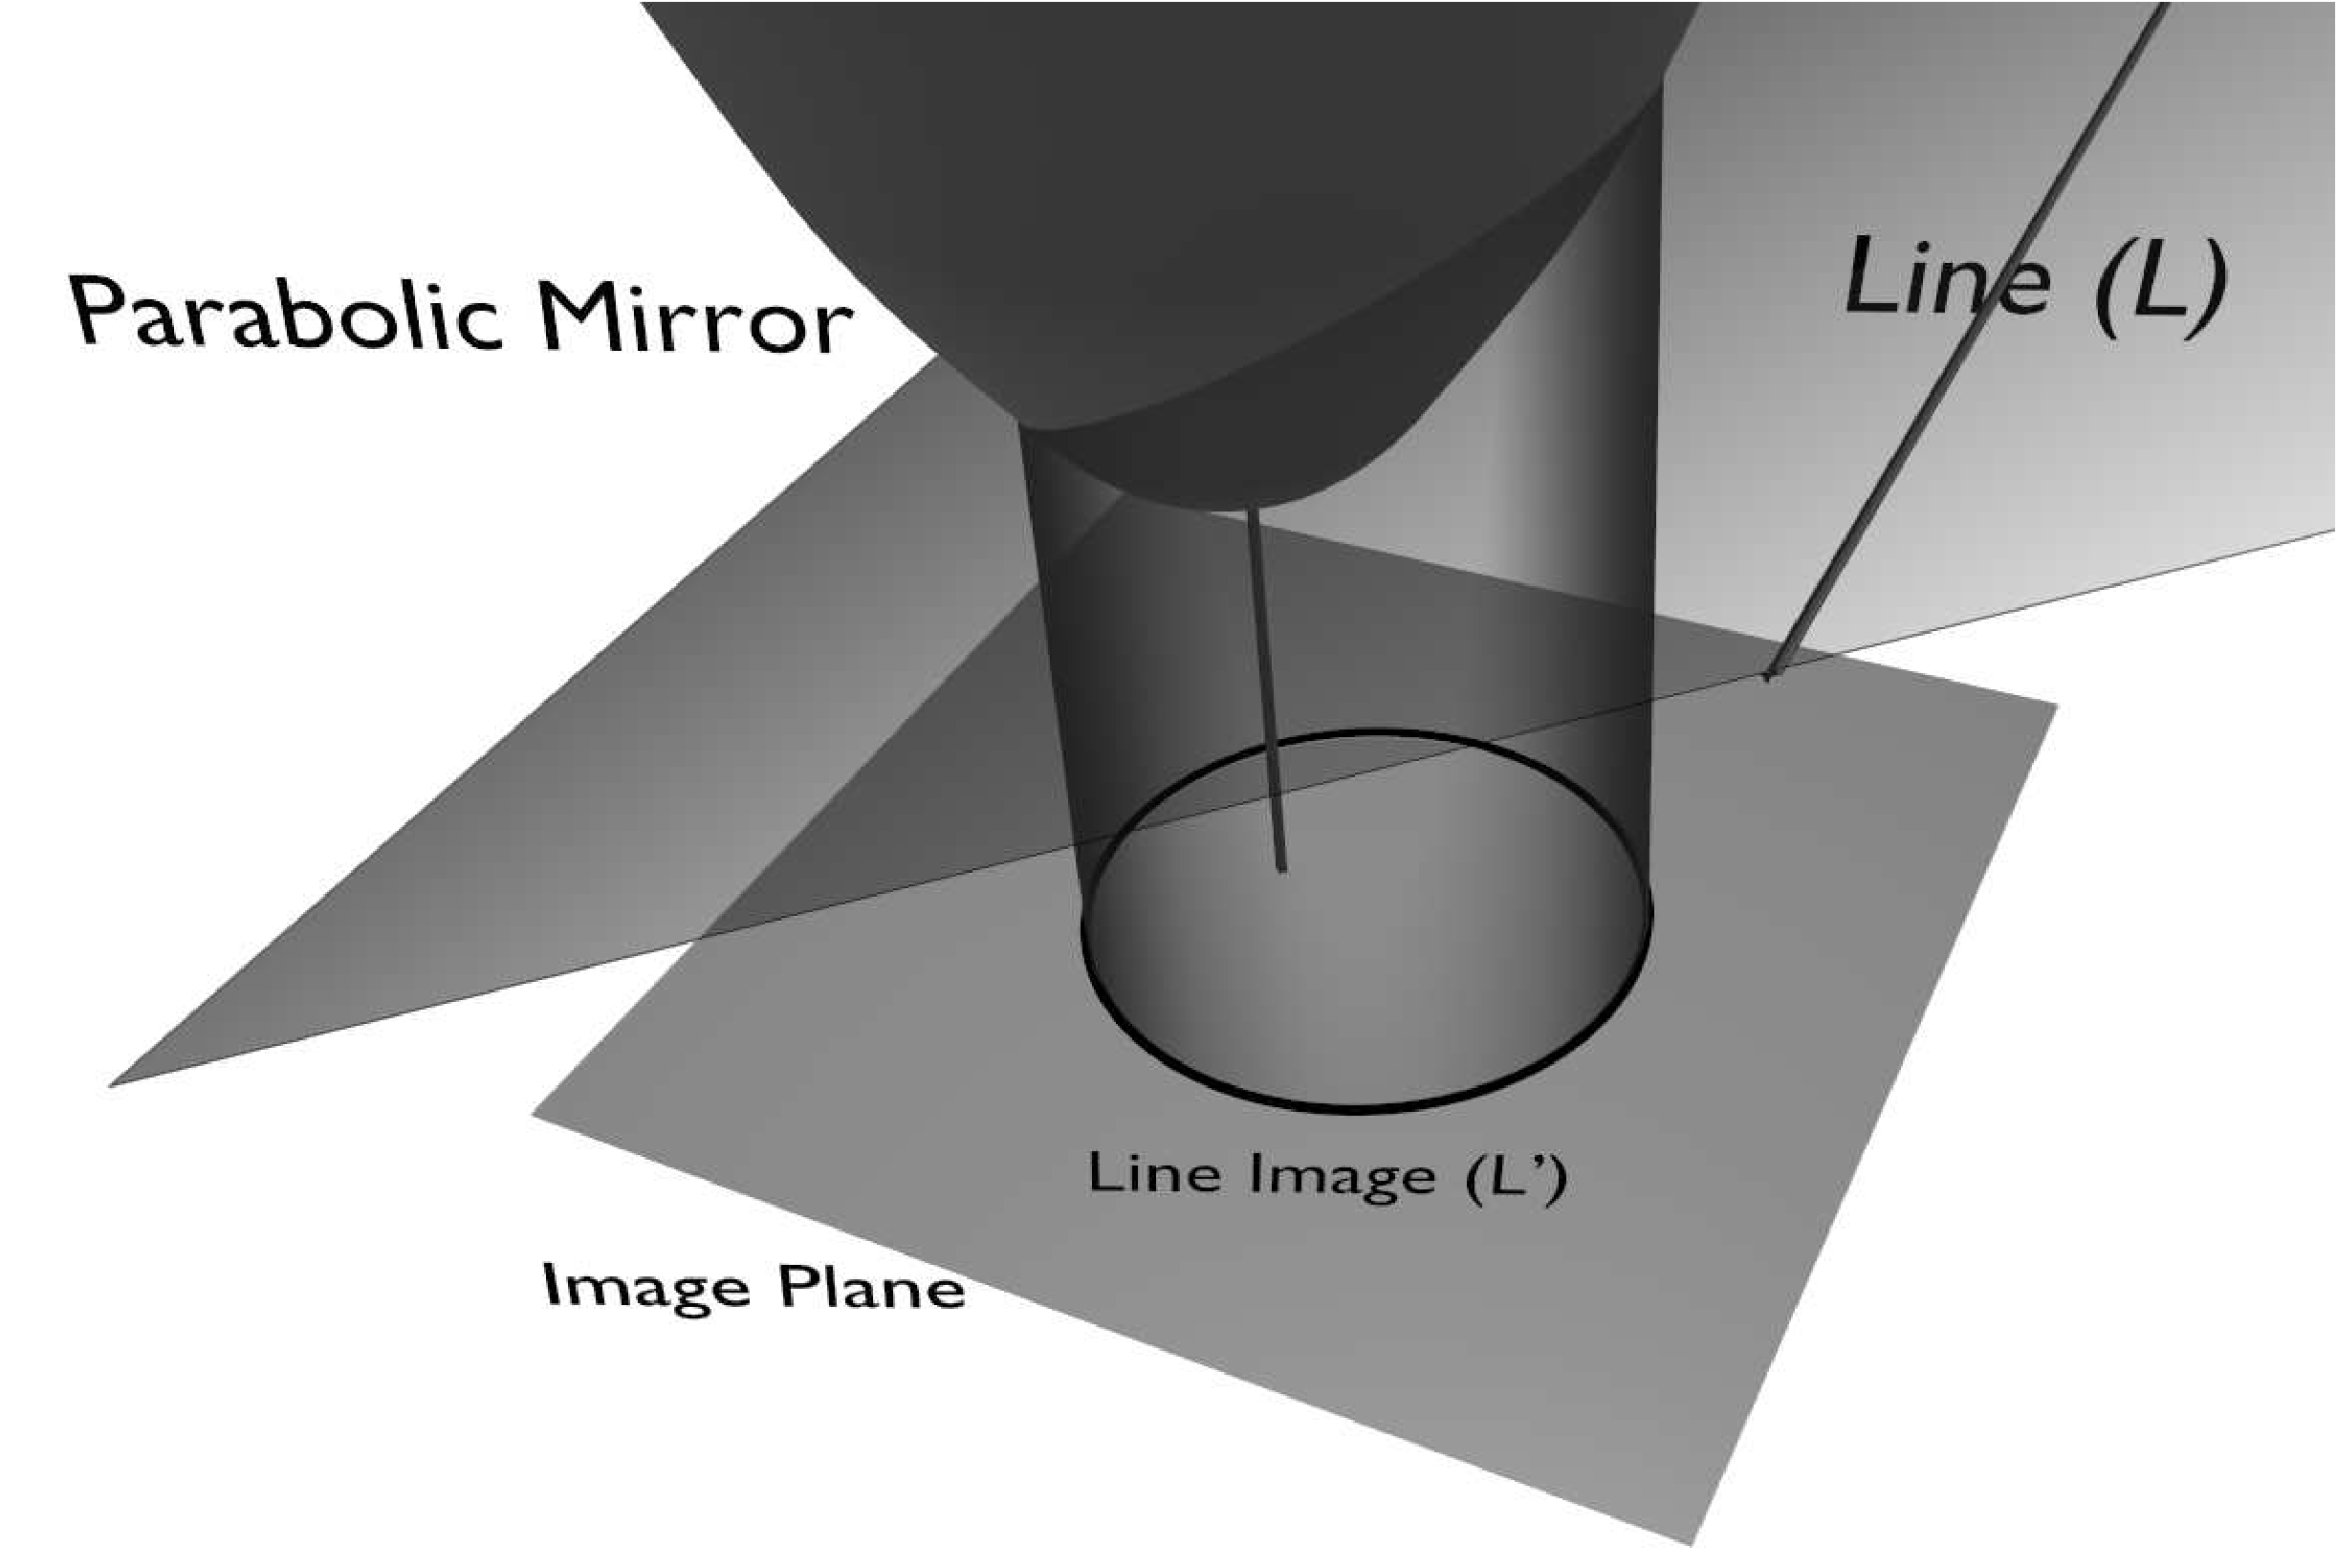
\includegraphics[height=8cm]{testparaboloid2}
\caption{Para-catadioptric Line Image Formation}
\label{fig:bob}
\end{figure}
As an illustration of the power of the techniques described above, let us consider the simple but
 useful question of what the image of a straight line in a parabolic mirror based Single View Point 
catadioptric (SVP Para-catadioptric) camera is.  This problem has been considered in a number 
of papers e.g.\ \cite{CAM:gd, CAM:YH04, CAM:BA03b, CAM:bclf} and is useful for calibration 
and scene reconstruction.

The setup in question is illustated in figure \ref{fig:bob}. With a parabolic
mirror the SVP constraint requires that all the rays from the mirror imaged by
the camera are parallel to the mirror axis and hence the camera is
orthographic. Let us consider the source of light forming an image at the point
$xe_2 + ye_3$.  As we are imaging with an orthographic camera, for the setup
shown, this ray is in the $e_1$ direction, which is axis of both the camera and the parabolic mirror.  The focus of the parabolic mirror is situated at the origin. 
\begin{eqnarray}  
S_1&=& \left[e_{23} + (xe_3 - ye_2)n\right]^* \nonumber
\end{eqnarray} 
This result is easily established if we consider the form of the dual of a line \cite{cgwcga}.
\begin{eqnarray}
L^* &=&	\hat{m}I_3 + [(a\wedge \hat{m})I_3]n\nonumber
\end{eqnarray}
with $\hat{m} = e_1$ (the ray's direction), $a = xe_2 + ye_3$ (a point on the ray) and $I_3 = e_{123}$.
This form is analogous to writing the line in terms of Pl\"{u}cker coordinates where 3 of the coordinates give the line's direction and the other 3 give its moment about the origin.

\chapter{Matrices}

We are interested in the reflection of this ray in the mirror.  This reflected ray, $S_2$ is found as
described in Section \ref{sec:Ref}.  
\begin{eqnarray} 
\label{eq:1} 
S_2 &=& \frac{1-x^2-y^2}2e_{145} -xe_{245} - y e_{345} 
\end{eqnarray}  
For this ray to be the image ray of a point on a line $L$ they must intersect and hence
\begin{eqnarray} 
\label{eq:2} L\vee S_2 &=& 0 
\end{eqnarray} 
As stated above, a line, $L$, with unit direction vector $\hat{m} = m_1e_1 + m_2e_2 + m_3e_3$ (such that $\hat{m}^2 = 1$) passing through the point $a = a_1e_1 + a_2e_2 + a_3e_3$, can be expressed as 
\begin{eqnarray} 
\label{eq:3} L &=& \left[\hat{m}I_3 + ((a\wedge \hat{m})I_3)n\right]^* 
\end{eqnarray} 

Subsituting equations \ref{eq:3} and \ref{eq:1} into \ref{eq:2} and rearranging, the condition obtained is 
\begin{eqnarray}
  \left(x + \frac{a_3m_1 - a_1m_3}{a_2m_3 -a_3m_2}\right)^2 + \left(y + \frac{a_1m_2 - a_2m_1}{a_2m_3 - a_3m_2}\right)^2 \nonumber&&\\- \left(1 + \left(\frac{a_3m_1 - a_1m_3}{a_2m_3 - a3_m2}\right)^2 + \left(\frac{a_1m_2 - a_2m_1}{a_2m_3 -a_3m_2}\right)^2\right) &=& 0
\end{eqnarray} 
As others have observed \cite{CAM:gd}, this is a circle ($L'$ in figure
		\ref{fig:bob}). A similar derivation can be used to establish
the image of a sphere in such a camera the only significant change being that
the resulting condition is the product of two separate circle equations,
    indicating an ambiguity which can trivially be resolved.  \nocite{CAM:bclf}

We may form a rotor $R$ using some generating
bivector $B$ via
\[
R = \exp(B).
\]
In 3d we may represent any rotation and
translation rotor as a $4\times4$ matrix $\mathcal{R}$ where
\[
\mathcal{R} = \left[
\begin{array}{cc}
\mathbf{A} & \mathbf{c} \\
                0 & 1
\end{array}
\right]
\]
and $\mathbf{A}$ is some rotation matrix and $\mathbf{c}$ is some
translation vector. The generator bivector, $B$, may itself be
parameterised in terms of a spatial bivector $P$ normalised s.t.
$P^2 = -1$, a scalar $\psi$ and a spactial vector $t$:
\[
B = \frac{\psi}{2} P + \frac{nt}{2}.
\]
Letting $P = p_1 e_{12} + p_2 e_{23} + p_3 e{31}$ and
$t = t_1 e_1 + t_2 e_2 + t_3 e_3$ we may represent $B$ via the
vector $\mathbf{c}$:
\[
\mathbf{c} = [ p_1 \; p_2 \; p_3 \; t_1 \; t_2 \; t_3 ]^T.
\]

Using the generator representation is useful since any 6d vector
$\mathbf{c}$ represents a valid generator and, hence, a valid rotor yet
the $4\times4$ matrix representation is useful for existing graphics
algorithms. This note aims to develop an algorithm for converting from
one to another with the proviso that converting from a matrix representation
to a generator is lossy since the matrix representation cannot uniquely
represent rotations by more the $2\pi$.

fsfsdsf
 sddgdgs sgsdg

\section{Theory}

Given a rotor $R$ generated by a bivector $B$ of the form above we may find
a function $h(\psi, P, t, p, \lambda)$ which applies the rotor generated
by $\psi, P$ and $t$ to the vector $p$:
\[
h(\psi, P, t, p, 1) = F^{-1} \left( R F(p) \tilde{R} \right)
\]
where $F(\cdot)$ is our usual vector to null-vector mapping.
After a little algebra\footnote{This phrase covers a multitude
  of sins...} we can see that the
following satisfies this requirement:
\begin{align}
h(\psi, P, t, p, \lambda) &=c^2p - s^2PpP - sc\left[pP - Pp\right] \nonumber \\
&\quad+ \lambda\left[ 
 \frac{kc+1}{2} t + \frac{kc-1}{2} PtP
- \frac{sk}{2} (tP - Pt)
\right] \label{eqn:defnh}
\end{align}
where $s = \sin(\psi/2)$, $c = \cos(\psi/2)$ and $k = \textrm{sinc}(\psi/2)$.
The function $h(\psi, P, t, p, \lambda)$ is clearly linear in $(p,\lambda)$ and so
we can find some $3\times4$ matrix $\mathcal{H}$, dependent on
$\psi, P$ and $t$, s.t.
\begin{equation}
\mathbf{e}^T 
 \mathcal{H} \left[
\begin{array}{c}
\mathbf{v}(p) \\ 1
\end{array} 
\right] = h(p, 1). \label{eqn:hi}
\end{equation}
where $\mathbf{e}^T = \left[ e_1 \; e_2 \; e_3 \right]$ and
$\mathbf{v} (p) = \left[ p\cdot e_1 ; p \cdot e_2 ; p \cdot e_3 \right]^T$. It is
fairly clear that
\[
\mathcal{R} = \left[
\begin{array}{cccc}
\multicolumn{4}{c}{\mathcal{H}} \\
                 0 & 0 & 0 & 1 
\end{array}
\right].
\]

\subsection{Finding $\mathcal{H}$ from a generator}

Given $A = a_{12}e_{12} + a_{23}e_{23} + a_{31}e_{31}$ and
$b = b_1e_1 + b_2e_2 + b_3e_3$, if we define
\begin{align*}
\mathbf{f}_1(A,b) &=
\left[ 
\begin{array}{ccc}
0 & a_{12} & - a_{31} \\
- a_{12} & 0 & a_{23}\\
a_{31} & - a_{23} & 0 
\end{array} 
\right]  
\left[ 
\begin{array}{c}
b_1 \\ b_2 \\ b_3
\end{array} 
\right]  
\\
f_2(A,b) &= (a_{12}b_{3} + a_{23}b_1 + a_{31}b_2) 
\end{align*}
it is easy to show directly that
\[
Ab =
f_2(A,b)\;e_{123} +
\left[ e_1 \; e_2 \; e_3 \right]
 \mathbf{f}_1(A,b)
\]
and
\[
bA =
f_2(A,b)\;e_{123} - 
\left[ e_1 \; e_2 \; e_3 \right]
\mathbf{f}_1(A,b)
\]
Hence
\[
bA - Ab = -
\left[ e_1 \; e_2 \; e_3 \right]
2\mathbf{f}_1(A,b).
\]
%Recalling $\mathbf{e}^T = \left[ e_1 \; e_2 \; e_3 \right]$
Defining
\begin{align*}
\mathbf{M}_1(A) &= \left[ 
\begin{array}{ccc}
0 & a_{12} & - a_{31} \\
- a_{12} & 0 & a_{23}\\
a_{31} & - a_{23} & 0 
\end{array} 
\right]  \quad\mathrm{and}\quad
\mathbf{v}(b) = \left[ 
\begin{array}{c}
b_1 \\
b_2 \\
b_3 
\end{array} 
\right]  
\end{align*}
we may rewrite equation \ref{eqn:defnh} as
\begin{align*}
h(\psi, P, t, p, \lambda) &= c^2\;\mathbf{e}^T\mathbf{v}(p) - s^2PpP + 2sc\;\mathbf{e}^T\mathbf{M}_1(P)\mathbf{v}(p) \\
&\quad+ \lambda\left[ 
 \frac{kc+1}{2} \mathbf{e}^T\mathbf{v}(t) + \frac{kc-1}{2} PtP
+ sk\;\mathbf{e}^T\mathbf{M}_1(P)\mathbf{v}(t)
\right].
\end{align*}
Similarly it is easy to verify that
\[
AbA = \mathbf{e}^T \mathbf{M}_2(A) \mathbf{v}(b)
\]
where
\[
\mathbf{M}_2(A)  =
\left[
\begin{array}{ccc}
a^2_{12} - a^2_{23} + a^2_{31} &  - 2a_{23}a_{31} & - 2a_{12}a_{23} \\
- 2a_{23}a_{31} & a^2_{12} + a^2_{23} - a^2_{31} & - 2a_{12}a_{31}  \\
- 2a_{12}a_{23} & - 2a_{12}a_{31} &  -a^2_{12} + a^2_{23} + a^2_{31} 
\end{array}
\right].
\]
We can now substitute into $h(\psi, P, t, p,\lambda)$ to obtain
\begin{align*}
h(\psi, P, t, p, \lambda) &= c^2\;\mathbf{e}^T\mathbf{v}(p) - s^2\;\mathbf{e}^T\mathbf{M}_2(P)\mathbf{v}(p) + 2sc\;\mathbf{e}^T\mathbf{M}_1(P)\mathbf{v}(p) \\
&\quad+ \lambda\left[ 
 \frac{kc+1}{2} \mathbf{e}^T\mathbf{v}(t) + \frac{kc-1}{2} \;\mathbf{e}^T\mathbf{M}_2(P)\mathbf{v}(t)
+ sk\;\mathbf{e}^T\mathbf{M}_1(P)\mathbf{v}(t)
 \right] \\
& = \mathbf{e}^T \left[ 
 c^2\;\mathbf{v}(p) - s^2\;\mathbf{M}_2(P)\mathbf{v}(p) + 2sc\;\mathbf{M}_1(P)\mathbf{v}(p) 
\right] \\
&\quad+ \lambda\mathbf{e}^T\left[ 
 \frac{kc+1}{2} \mathbf{v}(t) + \frac{kc-1}{2} \;\mathbf{M}_2(P)\mathbf{v}(t)
+ sk\;\mathbf{M}_1(P)\mathbf{v}(t)
 \right].
\end{align*}
Taking $\mathbf{I}_3$ as the $3\times3$ identity matrix, defining
\[
\mathbf{M}_3(P) = \frac{kc+1}{2} \mathbf{I}_3 
+ \frac{kc-1}{2} \;\mathbf{M}_2(P) + sk\;\mathbf{M}_1(P)
\]
%(note the sign change is due to 
%representing the matrix via its transpose for typograpsic convenience). 
and comparing with 
equation \ref{eqn:hi} we see that
\[
\mathcal{H} = \left[
 c^2\mathbf{I}_3 - s^2\;\mathbf{M}_2(P) + 2sc\;\mathbf{M}_1(P) \; ; \;
 \mathbf{M}_3(P)\mathbf{v}(t)
\right]
\]
which is indeed a $3\times4$ matrix as required. The matrix $\mathcal{R}$ may
now be found easily.

\subsection{Finding the generator from $\mathcal{H}$}

Firstly represent $\mathcal{H}$ as
\[
\mathcal{H} = [ \mathbf{A}\; ; \; \mathbf{c} ]
\]
where 
\[\mathbf{A} = c^2\mathbf{I}_3 - s^2\;\mathbf{M}_2(P) + 2sc\;\mathbf{M}_1(P)\]
and
\begin{equation}
\mathbf{c} = \mathbf{M}_3(P)\mathbf{v}(t). \label{eqn:b}
\end{equation}
Both $\mathbf{A}$ and $\mathbf{c}$ may be extracted from $\mathcal{R}$ easily.
Given the anti-symmetric and symmetric nature
of $\mathbf{M}_1(P)$ and $\mathbf{M}_2(P)$ it is clear that
\begin{align*}
\mathbf{A} + \mathbf{A}^T &= 
2\left[ c^2\mathbf{I}_3 - s^2\;\mathbf{M}_2(P) \right] \\
\mathbf{A} - \mathbf{A}^T &= 
4sc\;\mathbf{M}_1(P).
\end{align*}
If $sc \ne 0$ then we may recover $P$ by extracting elements of 
$\mathbf{A} - \mathbf{A}^{T}$ and renormalising. If $sc = 0$ then either
$s = 0$ or $c = 0$. If $s = 0$ it implies $\psi = 2n\pi$, $c = 1$ and 
therefore that 
$\mathbf{A} + \mathbf{A}^{T}$ should be the identity matrix and
we are free to choose $P$ as we wish. If $c = 0$ then $s = \pm 1$
and $\mathbf{A} + \mathbf{A}^{T} = 2 \mathbf{M}_2(P)$. We can then
extract $P$ from $\mathbf{M}_2(P)$. The sign of $s$, in this case, is arbitrary.

Assuming we have estimates for $s$, $k$ and $c$ from above, we may
estimate $\mathbf{M}_3(P)$ directly and hence recover
\[
\mathbf{v}(t) = \mathbf{M}^{-1}_3(P) \mathbf{c}.
\]
In practice we might wish to use LU decomposition or similar rather
than computing the matrix inverse if we deal with spaces with higer
dimensionality. Finally, given $s$, $c$ and $k$, an estimate for 
$\psi$ can be made. 

